\chapter{Design Iteration III}
\label{DesignIteration3}

\begin{flushright}{\slshape    
Making everything visible is great when you only have twenty things. \\
When you have twenty thousand, it only adds to the confusion.} \\ \medskip
    ---  Don Norman \cite{Norman1999}
\end{flushright}


The goal of the final iteration was to extend the scenarios developed in the previous iterations to a new domain, while still making use of the smart objects and concepts that have been developed thus far. This would allow for testing the general applicability of the concepts and techniques, while still being able to reuse some of the devices we have already developed.

\section{Requirements}

The use case scenario in this iteration revolves around a person's evening routine before falling asleep. It is a cross-domain scenario that extends the media domain into the sleep domain, and enables the exchange of different types of information. The domain of sleep was chosen for several reasons:

\begin{itemize}
\item Sleep is important for physical and mental well-being --- an important application area of our research group at TU/e.
\item The sleep domain is targeted by a number of recent \ac{IoT} devices that record and share data and can be accessed through their \acp{API}.
\item 	The sleep domain allows us to reuse some of our existing work on media sharing and lighting, extending it into a new domain.
\end{itemize}

In the fitness and sleep domains there are a plethora of devices that are well-known to the \ac{IoT} community but that are not interoperable, such as:

\begin{itemize}
	\item the Withings WiFi body scale\footnote{http://www.withings.com/en/bodyscale}, that transfers body weight wirelessly to a computer or mobile device,
  	\item the Fitbit\footnote{http://www.fitbit.com/} and Nike FuelBand\footnote{http://www.nike.com/fuelband/} fitness monitors, that track activities using a built-in accelerometer, and
	\item the Zeo sleep monitor\footnote{http://www.myzeo.com}, that records sleep cycles using a head-mounted sensor.
\end{itemize}
 

Existing software applications targeted at these devices visualise the data coming from these devices. Our goal is to enable serendipitous interoperability, and we are interested in seeing what will happen when the data and capabilities are shared between these devices. For example, we could use the data coming from a sleep monitor to to change the behaviour of a light in the room, or the alarm on a mobile phone. We distinguish between a number of subdomains within the area of well-being, as shown in Figure \ref{Wellbeing}.

\begin{figure}[bth]
\begin{center}
	\digraph[scale=0.65]{Wellbeing}{
		node [shape=plaintext, fontsize=16];
		Wellbeing [label="Well-being"];
		{rank=same; Social; Physical; Mental}
		{rank=same; Fitness; Sleep}
		Wellbeing -> Social [arrowhead=None];
		Wellbeing -> Physical [arrowhead=None];
		Wellbeing -> Mental [arrowhead=None];
		Physical -> Fitness [arrowhead=None];
		Mental -> Sleep [arrowhead=None];
	}
	\caption{Sub-domains of well-being}
	\label{Wellbeing}        
\end{center}
\end{figure}

Several devices were used in Iteration III, including:

\begin{itemize}
	\item an Android smart phone -- Samsung Nexus S;
	\item an internet radio -- Logitech Squeezebox Radio;
	\item the lamp from Section \ref{Lamp};
	\item a sleep monitor -- Zeo Sleep Manager; and 
	\item an Android tablet -- Samsung Galaxy Tab 10.1 WiFi.
\end{itemize}

We purposefully did not define a narrative for this design iteration, to refrain from only implementing the functionality described in the narrative. Instead, we looked at the meaningful ensembles we could create with the devices, attempting to allow for \emph{emergent functionalities} to surface by sharing device capabilities and interaction events.

The design iteration was implemented in the master bedroom of the Context Lab of TU/e, a lab with a setting that resembles a real home. Implementing the setup in an environment that allowed us to see its behaviour and implications in a realistic setting, gave insights that are regarded more valuable than obtained when building a setup on for example one's office desk. 


\section{Ontology design}
\label{OntologyDesign3}

In this iteration the earlier ontologies were consolidated into a single ontology. This helps make the ontology more manageable and removes the ``cruft'' of legacy statements that build up over time. 

The first design decision of this iteration was to introduce the notion of directionality. This gives additional meaning to the devices, which now need to be modelled as \emph{sources}, \emph{sinks} or \emph{bridges}. A music player is an example of a smart object that acts as a source when connected to a speaker, which in turn acts as a sink. When transitivity is introduced, a smart object can act as both a source and sink, which we define as a bridge. For example, consider the case where the speaker is connected to another speaker, which then also plays back the same music. The first speaker then acts as a bridge.

We can infer that a smart object is a sink using\\

\noindent Sink~\ensuremath{\equiv}~SmartObject~\ensuremath{\sqcap}~(functionalitySink~\ensuremath{\exists}~Functionality)\\\marginpar{See Table \ref{syntaxTable} on page \pageref{syntaxTable} for more details on the symbols and syntaxes used in this thesis.} 

where the symbol \ensuremath{\exists} is used to denote the existential restriction that \texttt{functionalitySink} is some kind of \texttt{Functionality}. A bridge is inferred using\\

\noindent Bridge~\ensuremath{\equiv}Sink~\ensuremath{\sqcap}~Source\\ 

A semantic transformer is a virtual component that is not physically addressable and is therefore not considered to be a smart object. However, it is a bridge, as it acts as both a source and a sink. A smart object is a physical object first, with a digital representation added later.\marginpar{Semantic transformers were first introduced in Section \ref{OntologyDesign2} and are discussed in more detail in Section \ref{SemanticTransformers}.}

Other areas where the ontology was improved include the modelling of device capabilities (Chapter \ref{DeviceCapabilityModelling}) and the modelling of events (Chapter \ref{EventModelling}). These improvements are discussed in more detail in the relevant chapters. 


%\section{Setting the time}
%It is reasonable to assume that modern networked devices will synchronize their clocks to a time server to display the actual time. Unfortunately, this is not the case. In our test setup, the internet radio synchronizes its clock with the local or remote server that it is connected to. The Android phone synchronizes its clock when it is connected to the GSM network 


\section{Device modifications}

In this iteration, we reused both the ambient lighting system from Section \ref{Lamp}, as well as the Connector object from Section \ref{Connector}. For the Squeezebox radio and Android devices new \ac{KP} software was developed.

\subsection{Squeezebox radio}

\begin{figure}
\centering
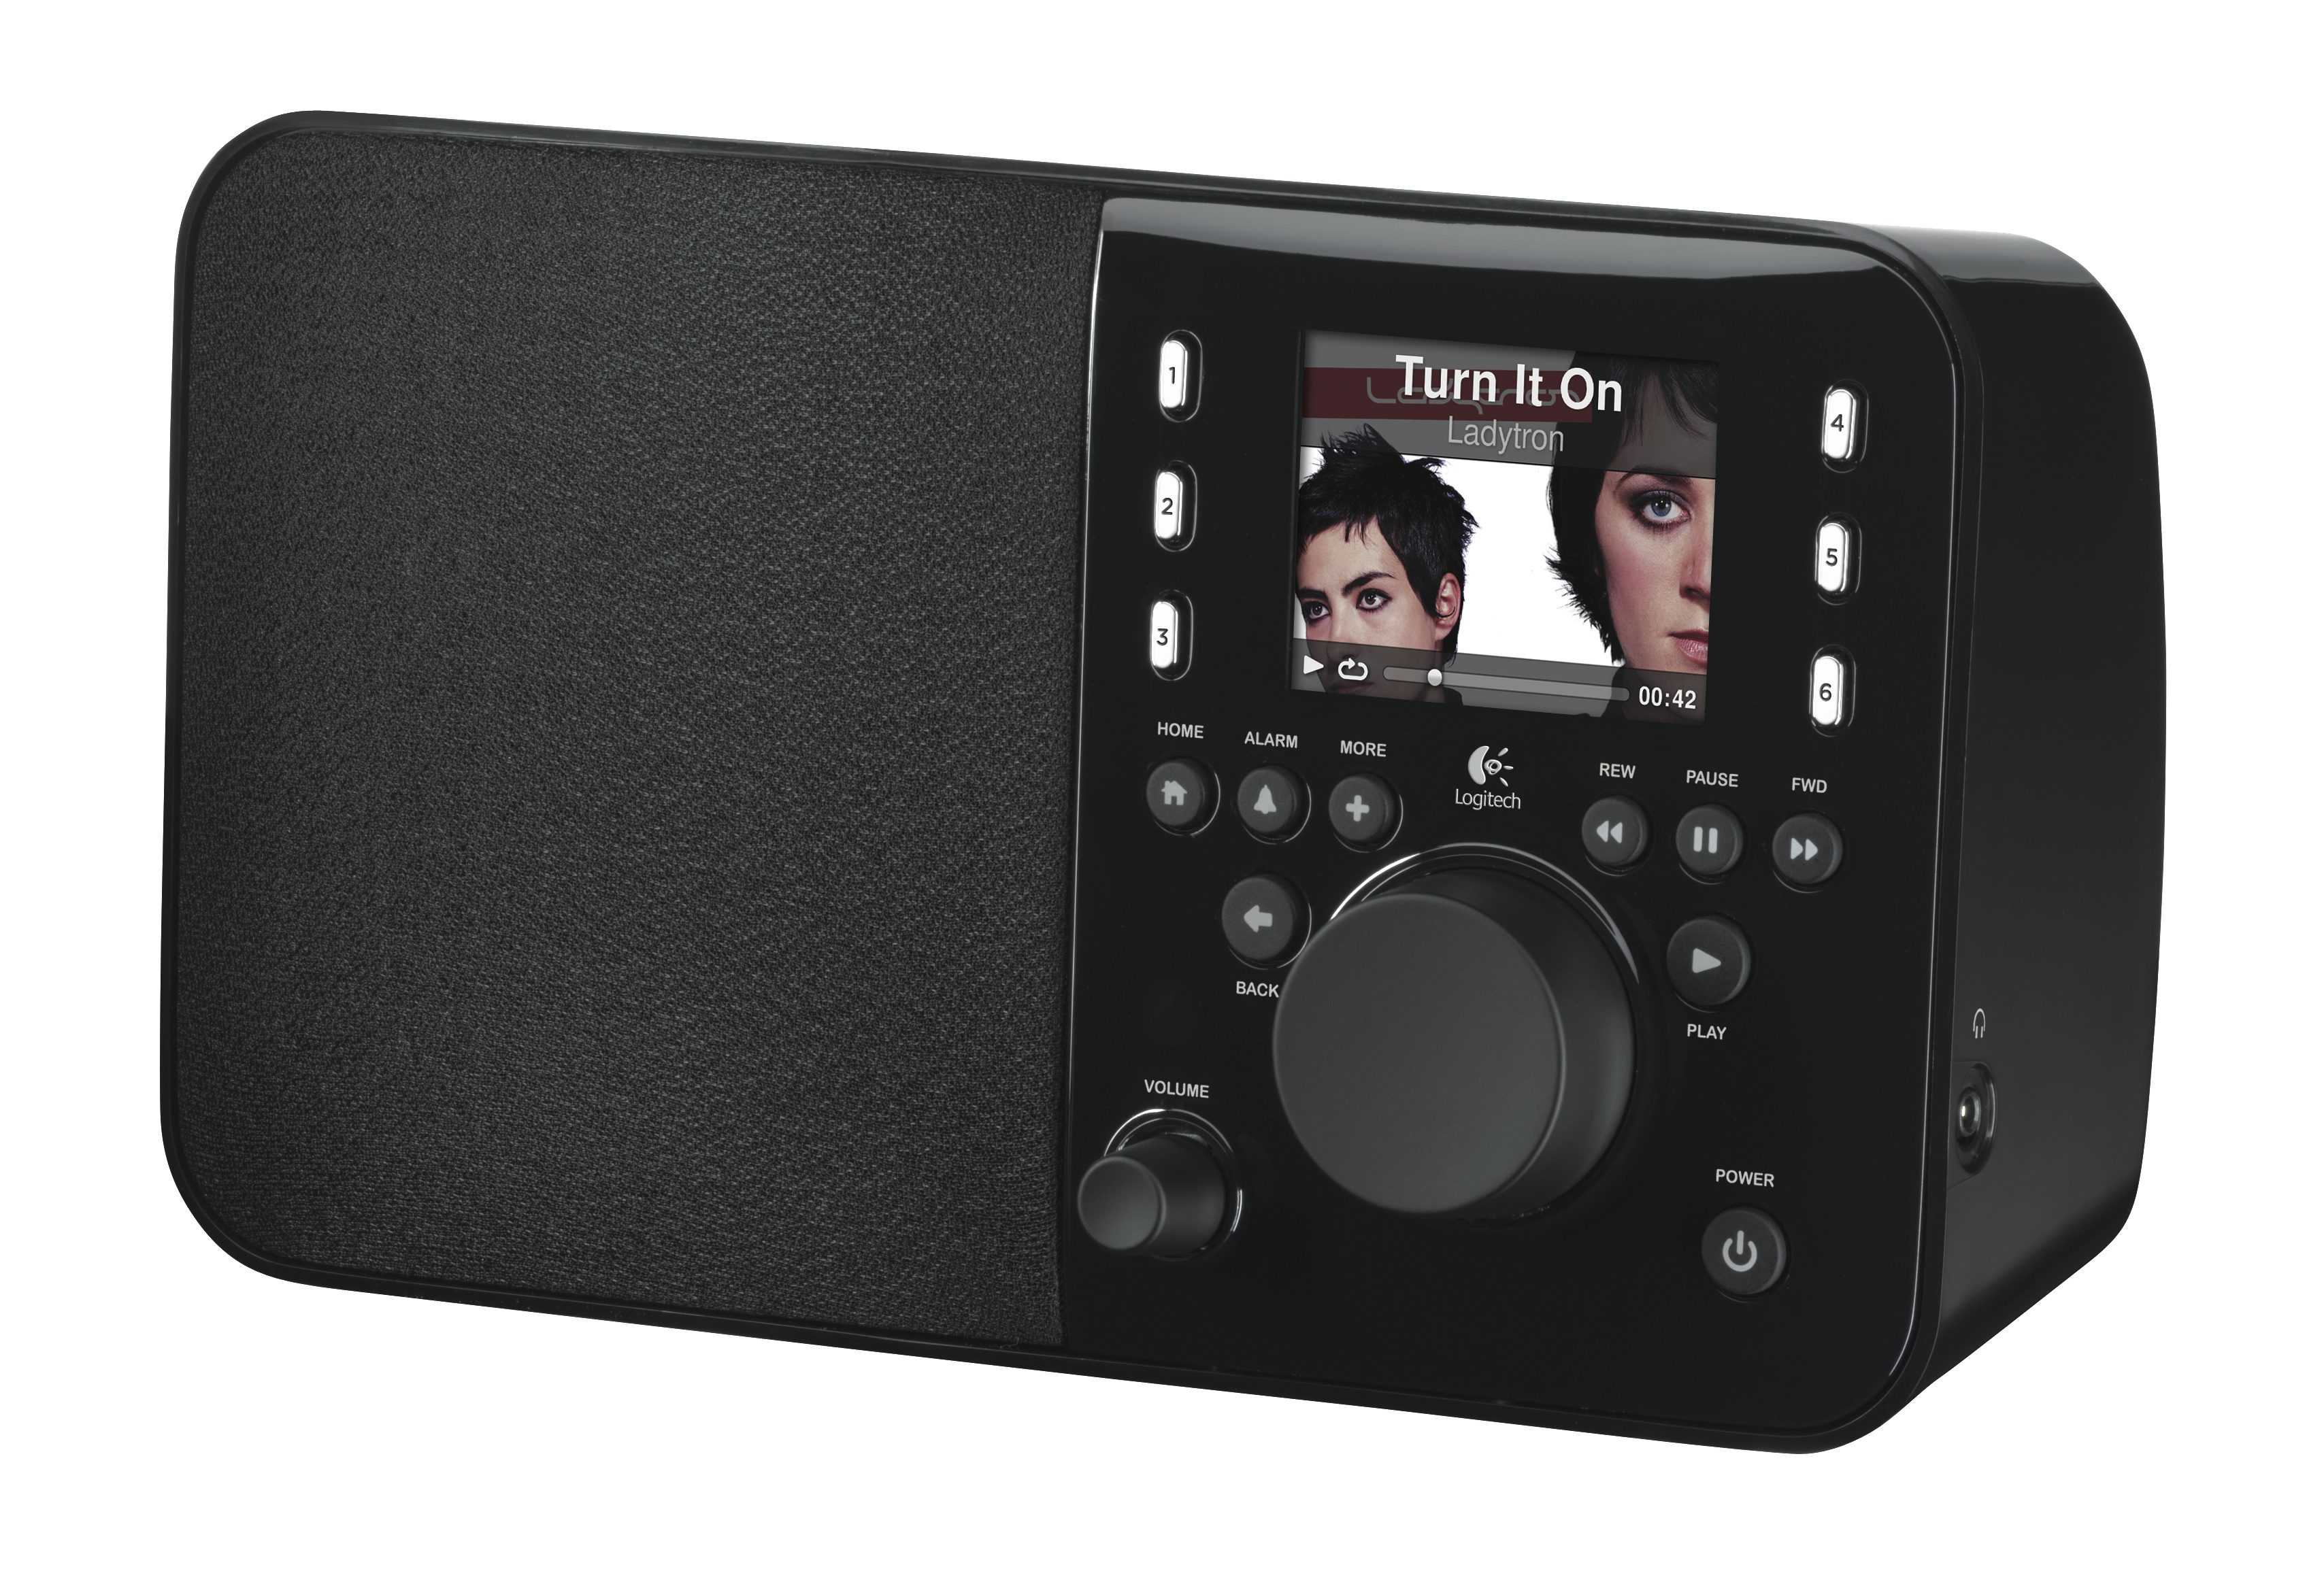
\includegraphics[width=300pt]{squeezebox}
\caption{Logitech Squeezebox Radio}
\label{squeezebox}
\end{figure}

The Squeezebox radio, shown in Figure \ref{squeezebox}, can be controlled via a Telnet interface over WiFi.\footnote{On Squeezebox Server, the interface documentation is available from \texttt{Help}~$\Rightarrow$~\texttt{Technical Information}~$\Rightarrow$~\texttt{The Squeezebox Server Command Line Interface} }. 
For example, the accepted parameters for setting an alarm are shown in Table \ref{SetAlarm}.

\begin{table}
    \myfloatalign
  \begin{tabularx}{\textwidth}{Xl} \toprule
    \tableheadline{Parameter} & \tableheadline{Description} \\ \midrule

    \texttt{dow} & Day of week (0 -- 6, starts on Sunday) \\
	\texttt{time} & Time since midnight in seconds \\
	\texttt{repeat} & 1 or 0 \\
	\texttt{volume} & 0 -- 100 \\
	\texttt{url} & Squeezebox Server \ac{URL} of alarm playlist \\
	\texttt{id} & The ID of an existing alarm (optional for new alarms) \\
    \bottomrule
  \end{tabularx}
  \caption{Accepted parameters for Squeezebox \texttt{alarm} Telnet command}  \label{SetAlarm}
\end{table}

On startup, the Squeezebox \ac{KP} connects to the smart space, registers the capabilities of the device, checks for existing connections and listens for new connections. It also subscribes to new system events.\marginpar{System events are discussed in more detail in Chapter \ref{OntologyEngineering}.} It then connects to the Squeezebox device via the Telnet-over-WiFi interface, subscribes to new events generated by the device and enters an event loop.


When a new alarm is set on the device, the \ac{KP} converts the date and time to \ac{XSD} format and generates a new \texttt{AlarmSetEvent}. When an alarm is triggered, an \texttt{AlarmAlertEvent} is generated. If the alarm is dismissed on the device, an \texttt{AlarmEndEvent} is generated. When an alarm is deleted, an \texttt{AlarmRemoveEvent} is generated.

When an \texttt{AlarmSetEvent}, \texttt{AlarmRemoveEvent}, \texttt{AlarmEndEvent} is received from another device, the corresponding action is performed on the device. \marginpar{Media events were introduced in Section \ref{MusicPlayerKP}.}The device also responds to media events like \texttt{PlayEvent}, \texttt{PauseEvent} and \texttt{PlayEvent}.


\subsection{Android mobile devices}

\begin{figure}
\centering
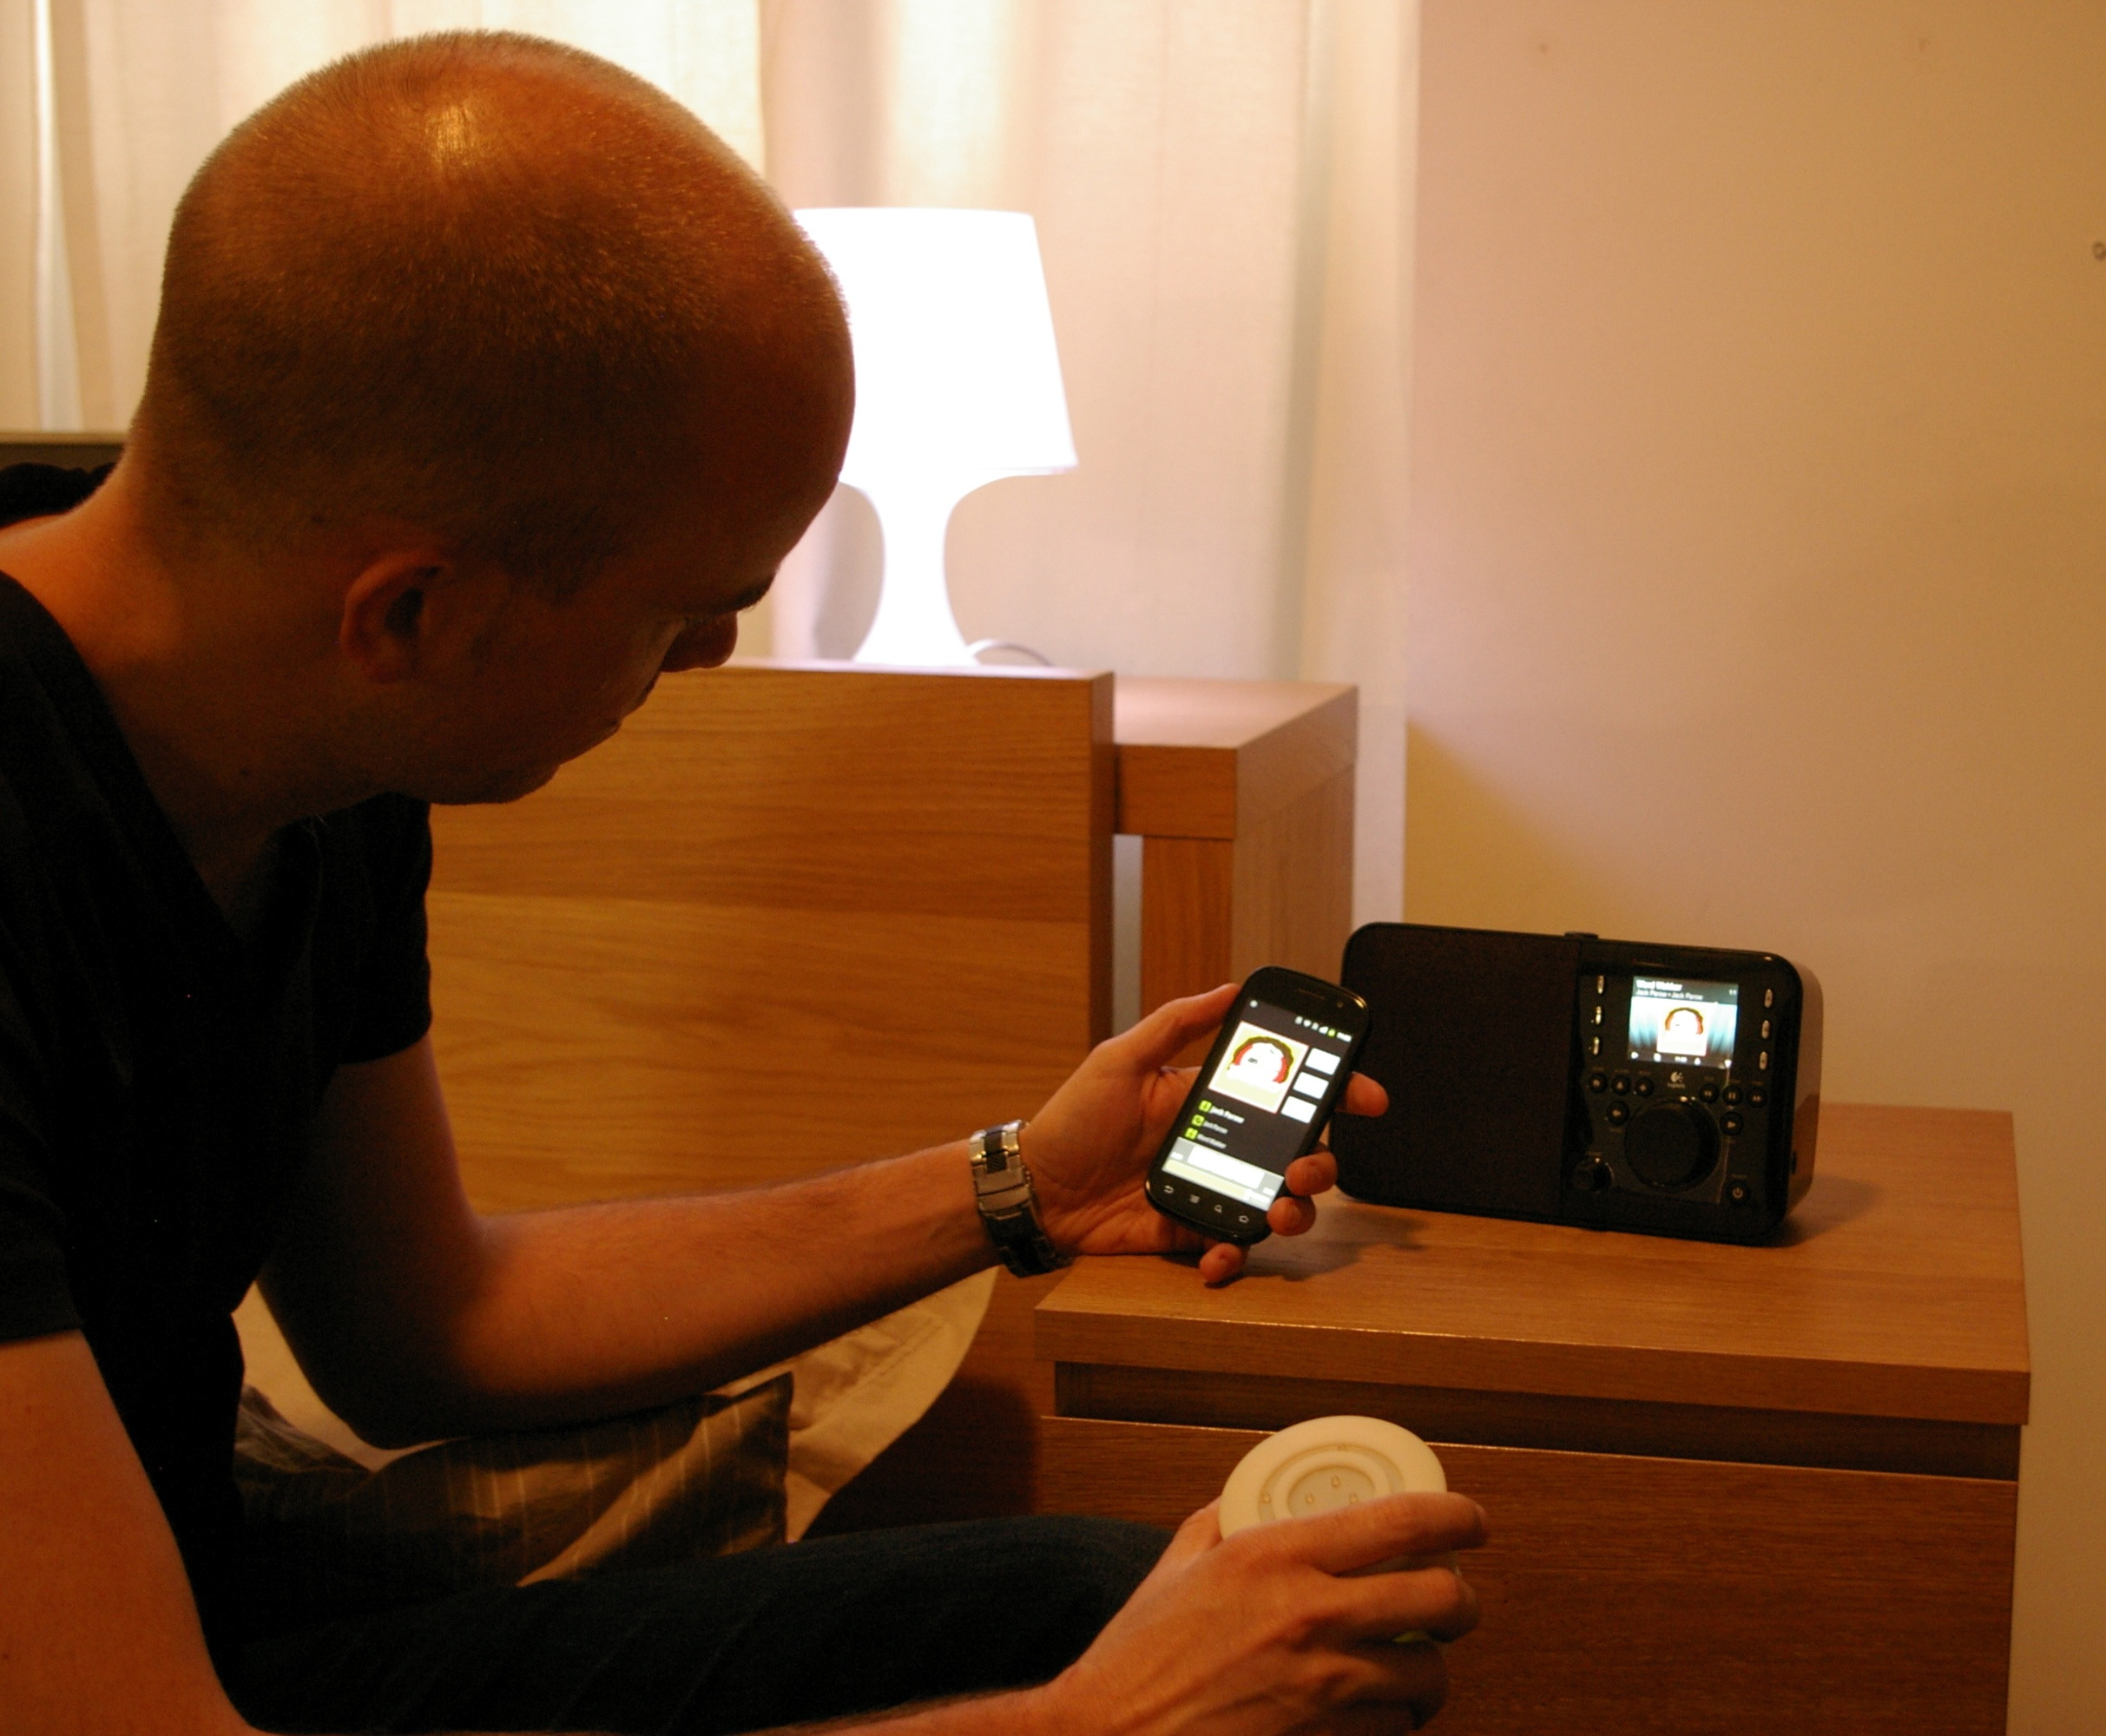
\includegraphics[width=300pt]{nexus}
\caption{Playing music from the phone on the Squeezebox radio}
\label{nexus}
\end{figure}

\marginpar{The \ac{KP} developed for the Android devices was tested on both the Google Nexus S phone and the Samsung Galaxy Tab.}
To improve software reuse and not reinvent the wheel, we wanted to make use of the stock applications on the phone, like the Clock app and the Music app (shown in Figure \ref{nexus}), instead of developing our own. On Android, it is possible to run a service as a background process that listens for events generated by other applications. A \emph{broadcast receiver} listens for \emph{broadcast intents}, which are public intents broadcast from activities to registered receivers. A receiver registers for a broadcast intent by listing it in its intent filter in the manifest file.\marginpar{Android activities run inside applications.} Broadcast intents sent by Android applications can be received by all other applications, which is done by creating a broadcast receiver. 

When the alarm is triggered in the alarm app on the mobile phone, a \mint{java}|com.android.deskclock.ALARM_ALERT| broadcast intent is generated. 

A broadcast receiver handles such an intent using 

\begin{minted}{java}
@Override
protected void handleBroadcastIntent(Intent broadcastIntent) {
	String action = broadcastIntent.getAction();
	if(action.equals("android.intent.action.ALARM_ALERT")) {
		addEvent("AlarmAlertEvent");
	}
}
\end{minted}

\marginpar{The alarm app on the Google Nexus S phone is called \texttt{DeskClock} and was developed by Google. There also exists a version for earlier Google phones called \texttt{AlarmClock}.}	
Note that this intent is not supported by all Android devices, as different devices may have different default alarm applications. It did, however, work on both the Google Nexus S phones and Samsung Galaxy tablets that we tested. To determine when an alarm was changed, we made use of the \mint{java}|android.intent.action.ALARM_CHANGED| broadcast intents. It is also possible to read the next alarm that will triggered from the system settings, using \mint{java}|System.Settings.NEXT_ALARM_FORMATTED| To determine if a song is being played using the Android Music app, we used the \mint{java}|com.android.music.playstatechanged| broadcast intent.

\marginpar{The Lighted Greenroom pattern was introduced by Komatineni et al. \cite{Komatineni2011} to simplify interacting with the Android wake lock.}
We used a Lighted Greenroom \cite{Komatineni2011} pattern to launch a long-running service from a broadcast receiver, without the operating system throwing an \ac{ANR} message. \ac{ANR} specifies a 10-second response limit for a broadcast receiver, after which it is deemed unresponsive. By launching a separate service that handles generation of events based on broadcast intents, we have a workaround to this problem. This allows us to listen for broadcast intents from applications like the music player and the alarm clock.
%(e.g. \texttt{com.android.music.playstatechanged}) and the alarm clock (\texttt{android.intent.action.ALARM\_CHANGED})

\subsection{Wakeup experience service}

In the sleep use case, music can be shared between the smart phone and the internet radio. Alarms can be shared between the phone and the internet radio, the internet radio and the lamp as well as the phone and the lamp. Because the lamp has only \texttt{LightOn/LightOff} and \texttt{AdjustLevel} capabilities, the most basic functionality of the lamp responding to an \texttt{AlarmEvent}, would be to turn on at the time that the event occurs. However, a wakeup service can be connected that \emph{transforms} an \texttt{AlarmSetEvent} into a wakeup experience, sending a sequence of \texttt{AdjustLevelEvents} to the lamp. This wakeup service then functions as a semantic transformer, transforming one type of value into another in a meaningful way. Semantic transformers are virtual entities and therefore they do not have a physical presence, in contrast to smart objects that must have a physical representation. Therefore, the use of a semantic transformer is automatically inferred based on its capabilities, as it cannot be physically connected to other devices by the user. 

To create a wakeup service, an \texttt{AlarmSetEvent} would have to trigger an \texttt{AdjustLevelEvent} event with a \texttt{dataValue} that increases from 0 to 100 over a period of 30 minutes \emph{before} the alarm sounds. Another requirement is that it should work with any light and any alarm in the smart environment. 

%The Wakeup \ac{KP} is a type of semantic transformer, and transforms \texttt{AlarmSetEvents} into a series of \texttt{IncreaseLevelEvents} (which is a sub-property of \linebreak \texttt{AdjustLevelEvents}). However, this happens in a way that is designed by the developer of the \ac{KP} and as such, can be seen as a (digital) service. 

This wakeup service has similar functionalities as a Wakeup Light (e.g. as sold by Philips\footnote{http://www.philips.co.uk/c/wake-up-light/38751/cat/}) which means it starts increasing its light level over a 30 minute time-period, reaching full intensity (as calibrated) at the set alarm time. The semantic connection between the phone's alarm and the dimmable light is an example of how such a connection can have emerging functionality, which does not exist without the connection and the wakeup service.  

This opens up many possibilities for users, as they may connect other lights, and potentially even other devices such as a networked thermostat, to either the alarm or the dimmable lamp, creating their own wakeup experience. Whether such emerging functionalities are possible obviously depends on the way the smart objects are implemented. For example in our implementation, the dimmable lamp is described as a sink, which means it is only capable of accepting input. If it was described as a source as well, sharing for instance its on/off state or its current light value, it could act as a bridge and allow for more interesting configurations. %Users may also connect the sleep monitor as an alarm source, helping them to wake up at the right time in their sleep cycle.

\begin{figure}
\centering
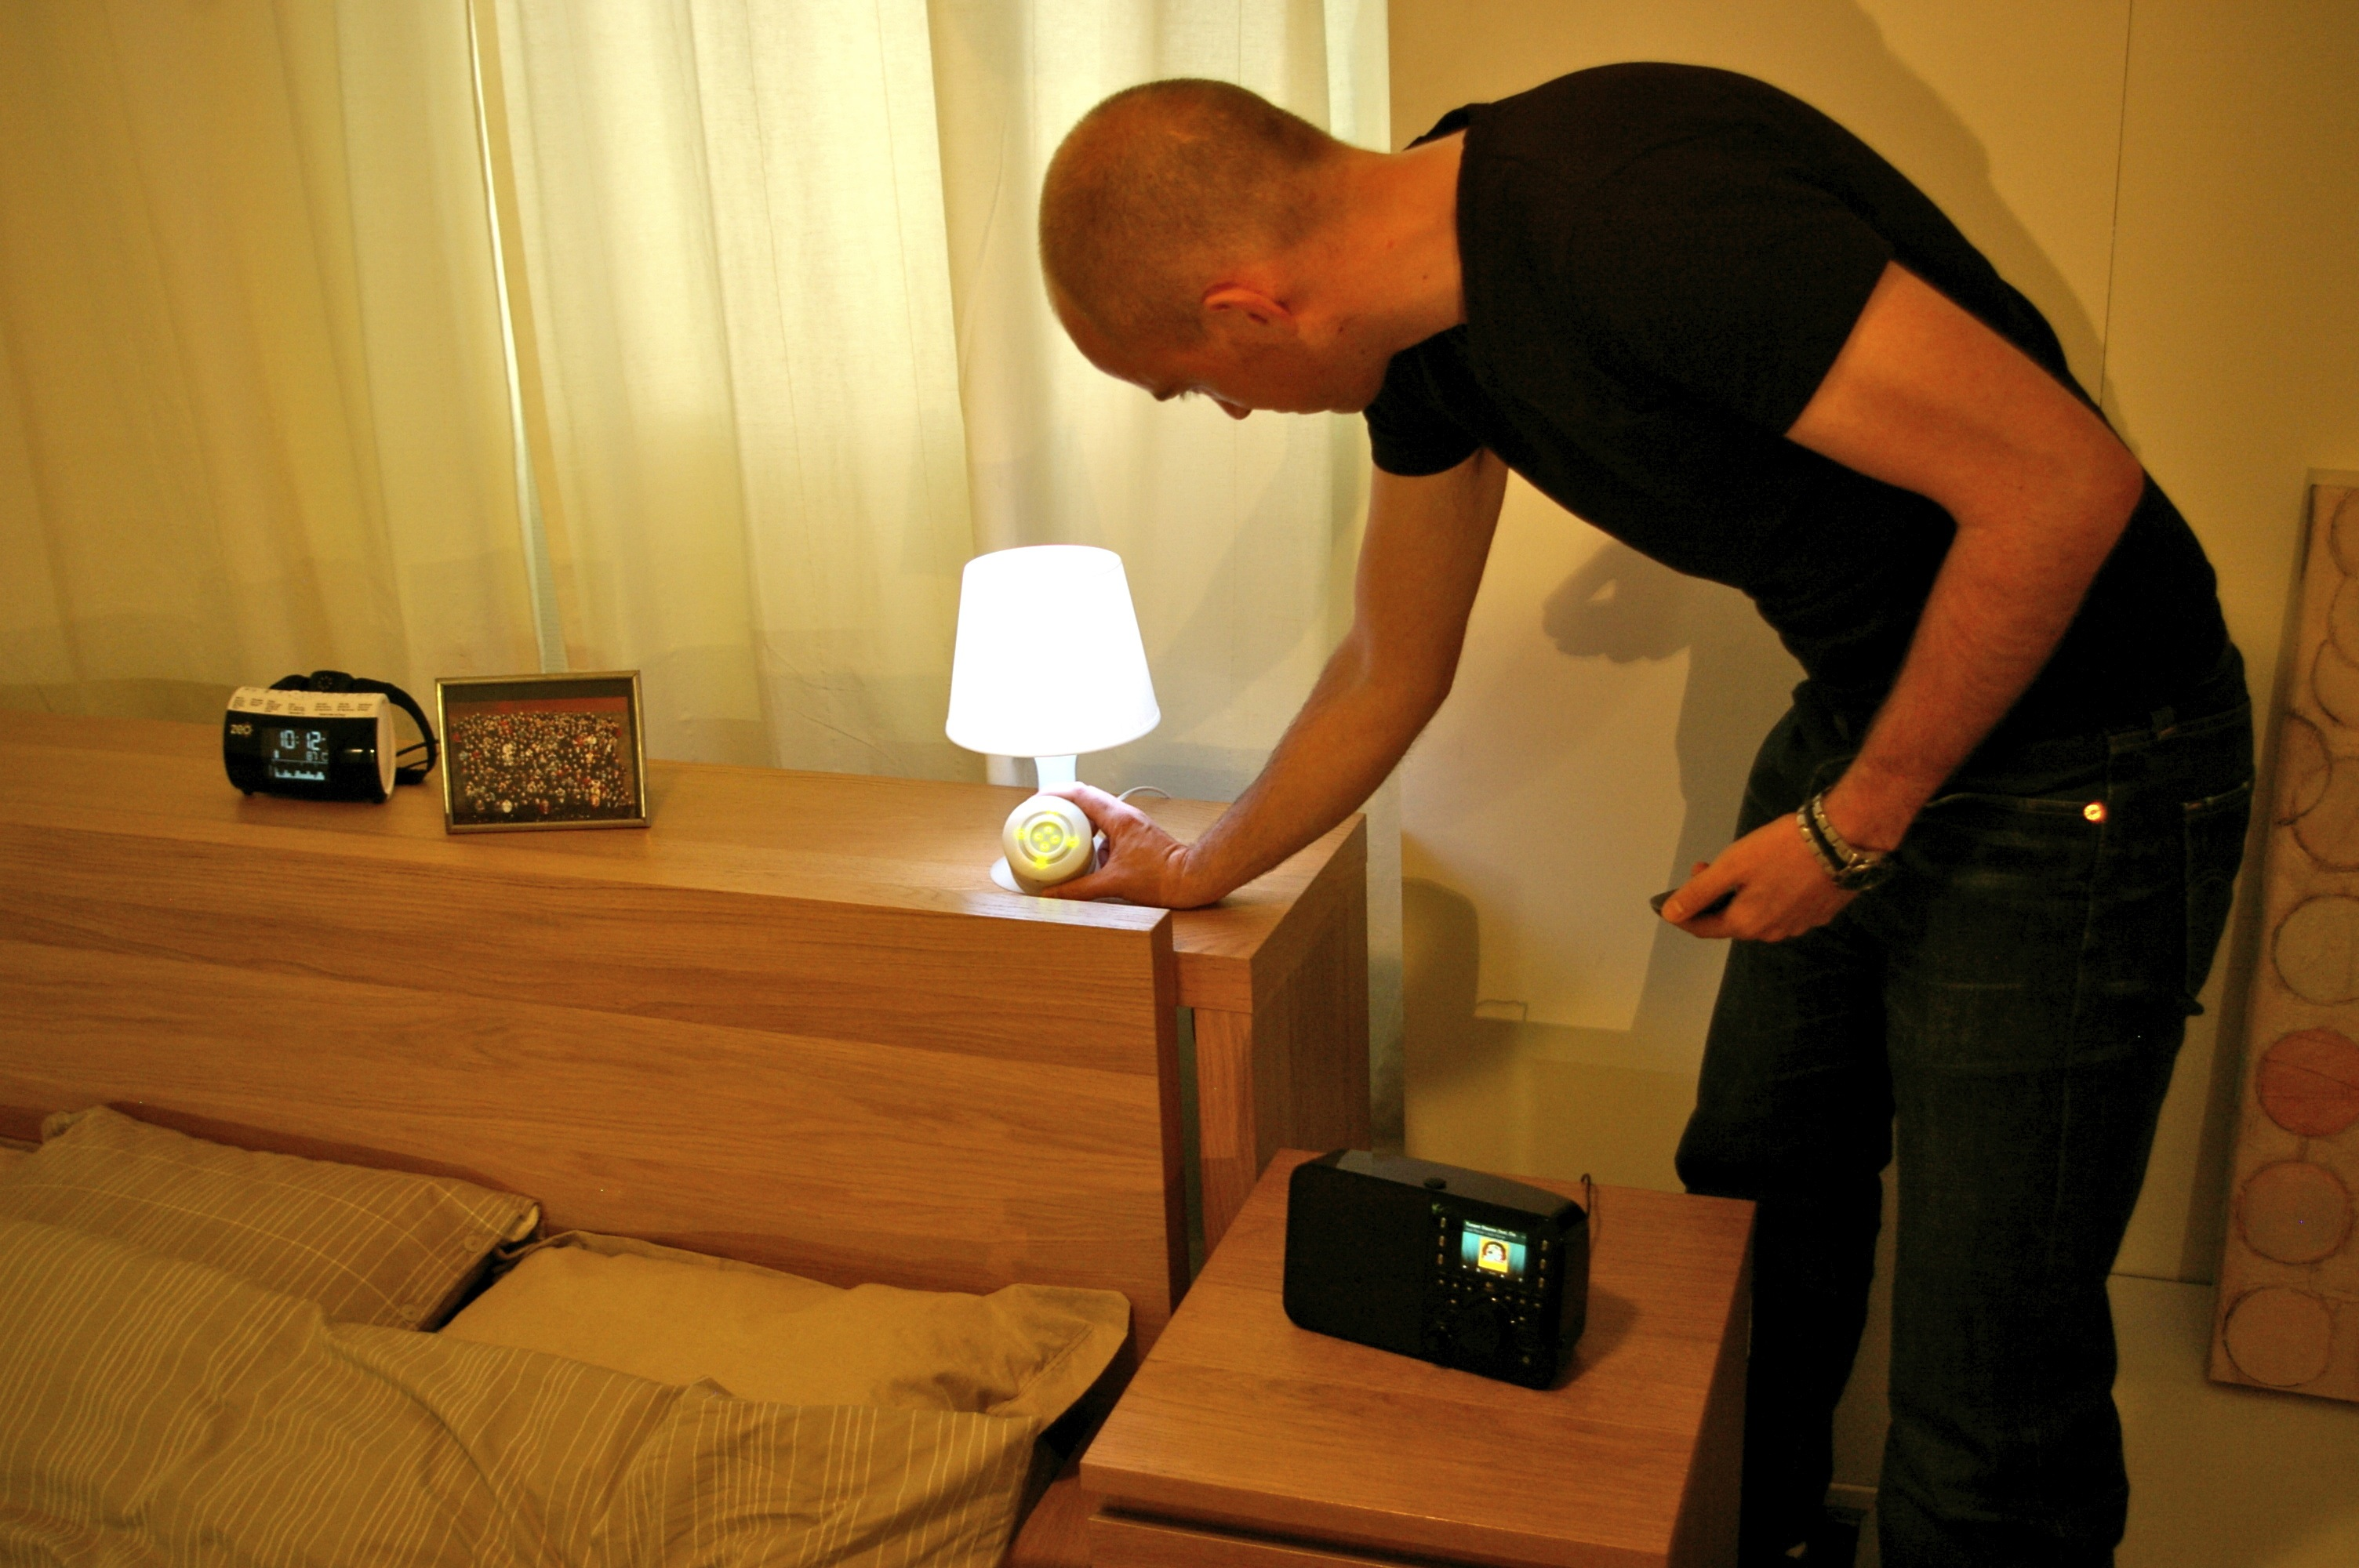
\includegraphics[width=300pt]{sleepscenario}
\caption{The sleep use case scenario, with the Zeo sleep monitor on the left, the dimmable light and the Connector object in the middle, and the Squeezebox on the right}
\label{sleepusecase}
\end{figure}

\subsection{Zeo}

The Zeo sleep monitor is shown on the left-hand side of Figure \ref{sleepusecase}. The Zeo headband, shown in Figure \ref{headband}, uses three silver conductive fabric sensors to collect \ac{EEG} signals while a person is sleeping. The signals are amplified and features are extracted using a \ac{FFT}. An \ac{ANN} is then used to estimate the probability of a person being in a certain phase of sleep\cite{Rubin2009}. The sleep stages are Awake, \ac{REM} Sleep, Light Sleep, Deep Sleep or Undefined. 

\begin{figure}
\centering
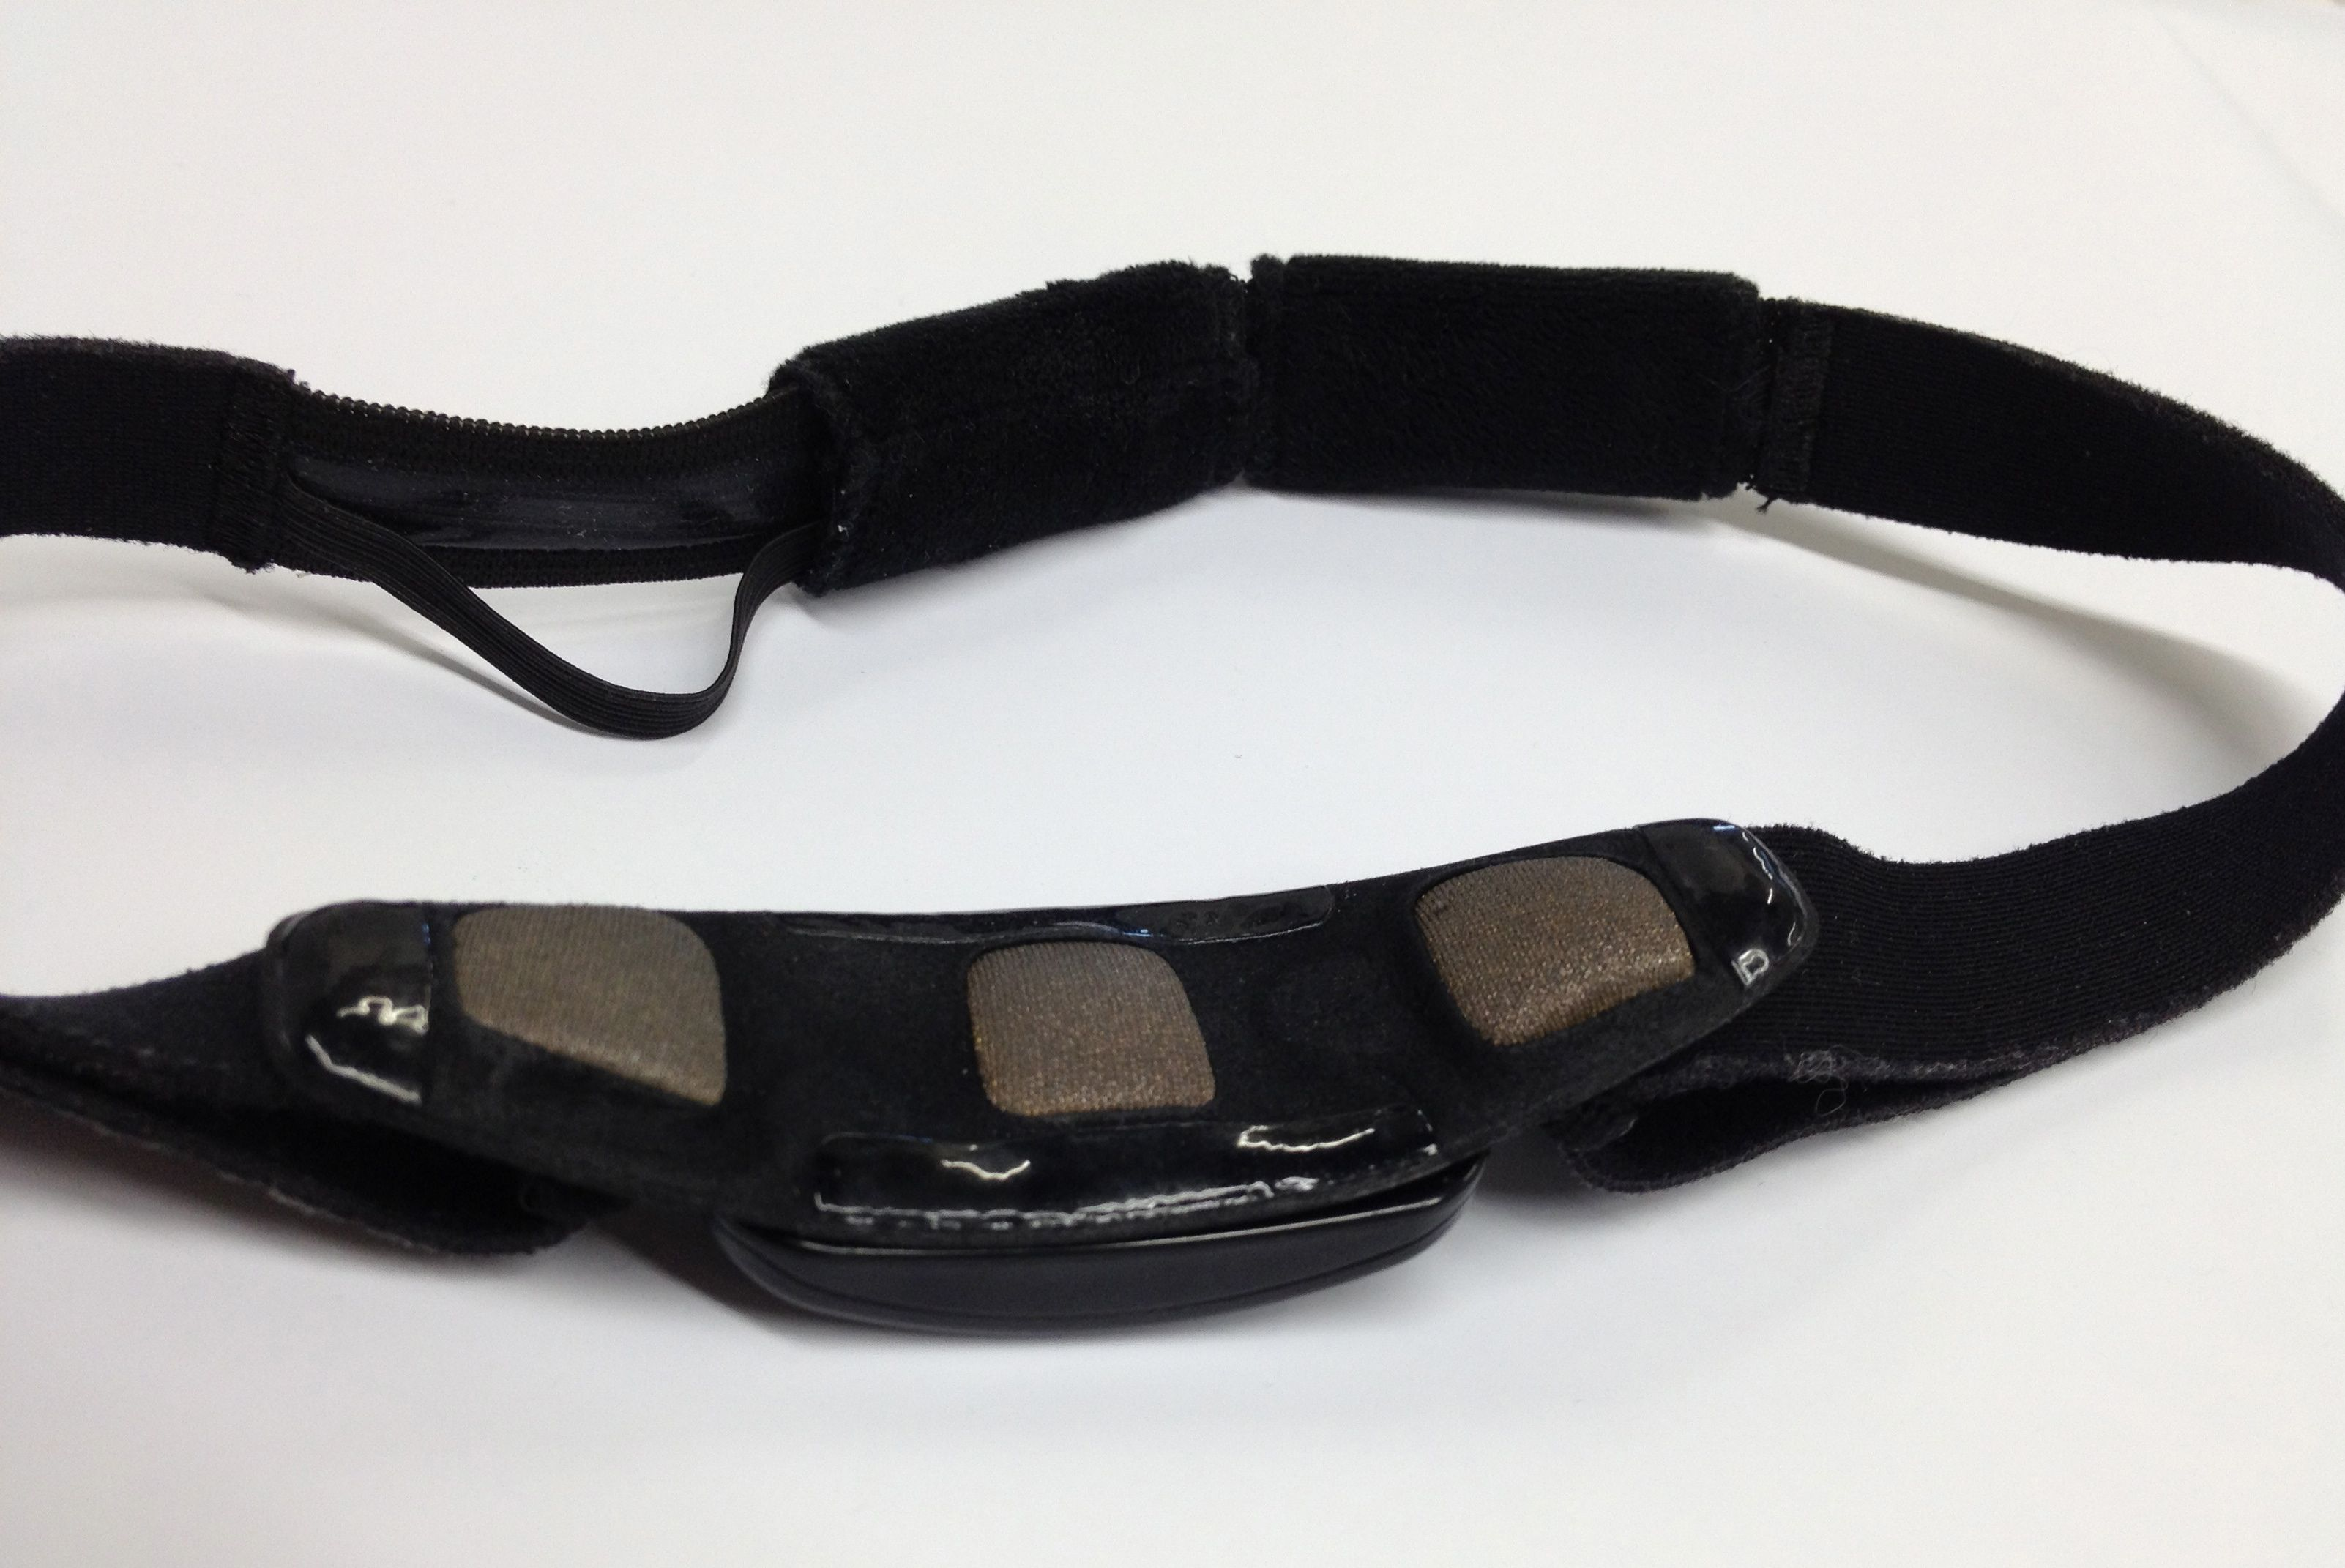
\includegraphics[width=300pt]{headband}
\caption{The Zeo headband}
\label{headband}
\end{figure}


Sleep data is stored on an SD card on the device and can be uploaded to the Zeo MySleep\footnote{http://mysleep.myzeo.com} website. Zeo created the Data Decoder Card library\footnote{http://developers.myzeo.com/data-decoder-library/} that allows developers to decode the sleep data without uploading the data to the MySleep website. We also built a USB cable that connects to a serial port on the back of the device. With this cable you can access the raw data coming from the headband sensor. %-- a diagram indicating how the USB cable should be connected to the Zeo is shown in Figure \ref{zeoBack}.

% \begin{figure}
% \centering
% 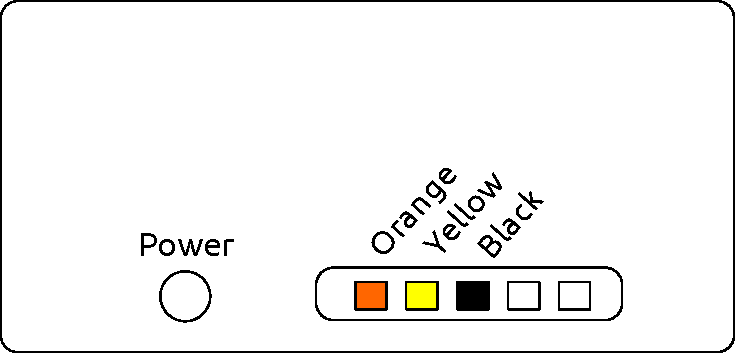
\includegraphics[width=300pt]{ZeoBack}
% \caption{Connecting a USB cable to the debug port of the Zeo sleep monitor}
% \label{zeoBack}
% \end{figure}

When the device is connected via a USB cable, we have real-time access to the generated events. Events that could be interesting to other smart objects in the environment include:

\begin{itemize}
	\item \texttt{NightStart} - time when first ``Awake'' hypnogram occurs
	\item \texttt{SleepOnset}
	\item \texttt{HeadbandDocked} and \texttt{HeadbandUndocked}
	\item \texttt{AlarmOff}, \texttt{AlarmSnooze} and \texttt{AlarmPlay}
	\item \texttt{NightEnd}
	%\item \texttt{NewHeadband}
\end{itemize}

% The Zeo Raw Data Library\footnote{http://sourceforge.net/projects/zeorawdata/} is a Python library to read raw data from the Zeo serial port, using the following commands:
% 
% \begin{minted}{python}
% 	from ZeoRawData.BaseLink import BaseLink
% 	from ZeoRawData.Parser import Parser
% 
% 	# Initialize
% 	link = BaseLink('/dev/ttyUSB0')
% 	parser = Parser()
% 
% 	# Add callback functions
% 	link.addCallback(parser.update)
% 	parser.addEventCallback(eventCallback)
% 	parser.addSliceCallback(sliceCallback)
% 
% 	# Start link
% 	link.start()
% \end{minted}
% 
A \ac{KP} was developed for the Zeo sleep monitor. Although it was not used as part of the final scenario, the Zeo shares its data like sleep states and alarm events in the smart space, which can be used by other devices.
 





\section{Implementation}
\label{D3Implementation}
  
\begin{figure}
\centerline{
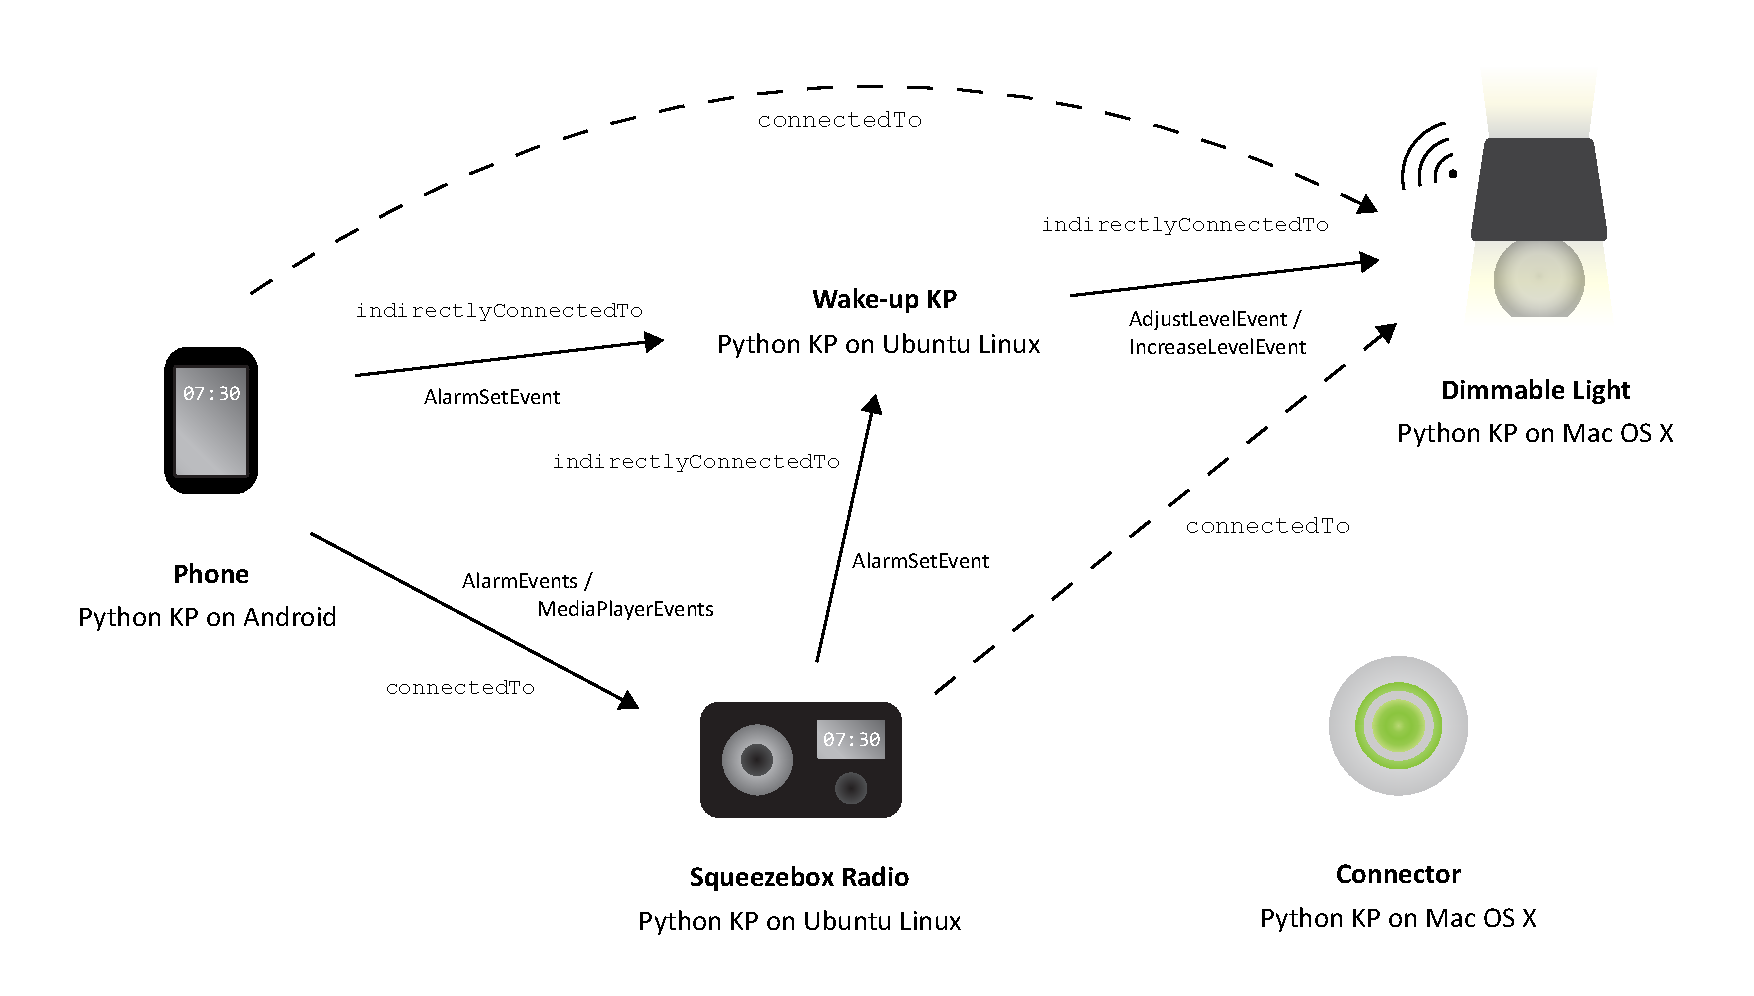
\includegraphics[width=450px]{sleepUseCase}}
\caption{An overview of the sleep use case}
\label{sleep}
\end{figure}\marginpar{In the sleep use case we did not make use of the Zeo and its \ac{KP} implementation. It was viewed as a backup device which could be used to introduce additional complexity to the system if necessary.}


%\subsection{Setup} %Method? perhaps a different heading
We started by implementing a very basic configuration, connecting the phone and the internet radio. Based on the capabilities of the devices, possible connections included sharing music player functionality and alarm clock functionality. After implementing the first basic functionalities, we gradually increased complexity by adding another smart object, the dimmable lamp, followed by the implementation of several types of interaction feedback.

% As an interface to semantic connections we used a smart object called the \textit{Connector} (TODO cite). The Connector device follows a tangible interaction approach, enabling users to physically select devices in their environment and directly view and manipulate the connections in a simple, universal way. It is a hand-held device that identifies devices by scanning RFID tags that are located on the devices themselves. By holding the Connector on top of the tag, users can explore the connection possibilities that are visualized with light segments located on top of the Connector. After holding the device in the RFID field for a moment, the device-ID is locked in and the other device to be connected can be selected in a similar fashion. With a push-to-click action a connection between two devices can be established. For removing an existing connection, the ring on the lower part of the device should be pulled until it clicks. Using the Connector and the semantic connections theory allowed us to shift our focus to how subtleties in design and interaction with the smart objects impact the overall user experience. Therefore, the design focus was not on the object interfacing with the connections but rather on the behaviour of the smart objects which are connected.

%\subsection{Implementation Examples}
%\label{section:implementationExamples}



%\subsection{Interaction with semantic connections}
%During the implementation phase, several changes were made to the Connector object to support the functionalities of the sleep use-case. In this section, the most important changes are discussed, as well as the limitations of the Connector's design and their implications for designing for interoperability in general.
%
%\subsubsection{Directionality}
%Although the Connector was originally designed to support the notion of directionality in the interaction with semantic connections, it was not implemented during our previous iteration. The two rings of the Connector's display signify input and output, or source and sink. Where in the previous iteration they indicated the selection of a first and then a second endpoint for the connection (which was symmetric) this was now changed to identify source and sink. The order in which the objects are physically identified is used to determine the direction of the connection. 
%
%Practically this means that the first object a user selects, should be the source object of a connection. When the smart object which is selected is not a source, this is indicated by means of feedback. 
%The same holds for the selection of the second object, which is required to be a sink. When the second object that is selected is not a sink, this is indicated by feedback.
%
%For exploring existing connection, the procedure to follow is similar. The order of selecting define the source and sink to query for an existing connection between the two and feedback is provided accordingly.  
%
%To help users understand why connections are not possible, e.g. their capabilities do not match, the first object is not a source, the second object is not a sink, or an error is returned, the connector should provide distinct feedback for each situation\footnote{The Connector already differentiates between connection possible, connection exists, connection is not possible and a state where both objects are scanned, but an error occurs (e.g. error in the KP, smart object is not subscribed to the SIB). In such cases, both rings remain orange.}. In case the first object is not a source, the outer ring flashed red (indicating it is a sink). When the second object is not a sink, the inner ring flashes red, indicating the object is a source. % explain why this mapping is chosen
%
%% add section on the insights that are gained e.g. limitation of design
%Introducing directionality with the current design of the Connector basically doubles the number of actions as between two given smart objects two connections instead of one may exist. This makes the required actions for more complex configurations cumbersome, and clearly shows the limitations of the current approach. A more comprehensive discussion on directions for a redesign are discussed in section \ref{chapVconnector}.

%\subsubsection{Transitivity}
%With directional connections implemented, the notion of transitivity defines some smart objects as \emph{bridges}. Bridges are different from sources and sinks when they are interacted with, as they behave both as a source and a sink. This becomes particularly clear when exploring existing connections. % add problems surfacing in the interaction.
%
%\subsubsection{Permanent and temporary connections}
%A notion of persistence for a connection was implemented in this iteration. When a source and sink are selected and a connection is possible, temporary connections (in contrast to regular connections; \texttt{connectedTo} relationships) were implemented to enable the use of \emph{preview events} (also see Section \ref{section:augmentedFunctionalFf} below). Temporary connections may also be created between the source and the sink when a possible connection is being explored. Therefore, while the system is in this state, the temporary connection can be used to exchange information. When the connection is confirmed, or when the state is cancelled, the temporary connections either become permanent, or are removed again.

%updates made to the connector

\subsection{Feedback and Feedforward}
\label{section:feedbackAndFeedforward}

\marginpar{In Van der Vlist's thesis \cite{Bram} there is a similar discussion on feedback, that focuses on some of the more user-centred aspects.}
In Section \ref{interactionFrogger}, where the Frogger framework of Wensveen \cite{Wensveen2005} was introduced, we also introduced the terminology of augmented and functional feedback/feedforward. We use feedforward to display a device's functional possibilities. We can use feedback to confirm user actions, using augmented feedback where direct functional feedback is not available.

When an alarm is set on the phone, augmented feedback should be given on all devices connected to the phone. For example, consider the setup in Figure \ref{phoneAlarmFeedback}, where the alarm is connected to both the lamp and the Squeezebox radio. 

\begin{figure}
\centering
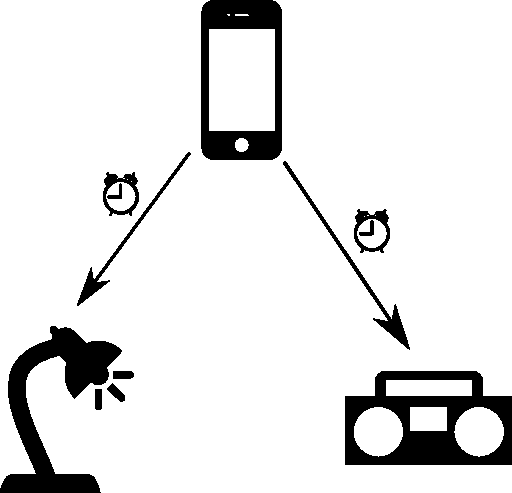
\includegraphics[width=250px]{phoneAlarmFeedback}
\caption{Alarm functionality of the phone shared with the radio and the lamp}
\label{phoneAlarmFeedback}
\end{figure}

Immediate feedback only makes sense when the event and its feedback coincide in time and modality (e.g. audio, visual). When the generated event is a \texttt{SetEvent}, the event itself will occur sometime in the future, so we generate the functional feedforward as augmented feedback instead. For example, for an \texttt{AlarmSetEvent} we generate a $1s$ alert sound on the Squeezebox radio as augmented feedback, providing functional feedforward of what will happen when the alarm is triggered. We also provide visual augmented feedback by displaying a popup message on the display for a few seconds. On the lamp feedback is given in the form of a short light pulse to confirm that it has been notified as well.

\marginpar{Many solutions for interconnecting devices often employ the \emph{vendor lock-in} strategy, which enables manufacturers to have full control over their ecosystem of products and the resulting user experience.}
Feedback and feedforward need to be carefully designed when smart objects are interconnected. However, as the smart objects themselves are unaware of each other and, at development time, their designers cannot anticipate what other devices users may connect the smart objects to, the total user experience cannot easily be designed. In this section we will describe how feedback and feedforward were used to enhance the user experience and enable devices that are in-fact unaware of one another, appear to show awareness of each other to their users. 

\subsubsection{Augmented and functional feedforward}
\label{section:augmentedFunctionalFf}
For semantic connections, functional feedback and feedforward can only be considered for the combination of source and sink. The source object has functional feedforward that may communicate its function. Only when both the source and sink object have been identified, is functional feedforward available for the semantic connection. Important to note is, that  functional feedforward is derived from the intersection of functionalities of both the source and the sink. These functionalities could be ambiguous, as both source and sink may be multifunctional. If this is the case, users should make explicit what information or data they want to exchange by selecting the desired mode on the source object (e.g. selecting the alarm application on your smart phone to share the alarm time or go to a picture viewer when pictures should be exchanged), restricting the possibilities. If this is not possible, or a multifunctional smart object is connected when it is in idle mode, semantic reasoning could be used to match all meaningful capabilities of the source and sink objects.

Whenever users wish to make a connection, they have certain expectations. We can employ functional feedforward to influence these expectations. Additionally, we can enhance the user's understanding by explicitly adding augmented feedforward (i.e. augmented \emph{functional} feedforward in contrast to augmented \emph{inherent} feedforward). In the sleep use-case we employed augmented feedforward in the process of exploring connection possibilities i.e. before the connection is made. We do this by giving a \emph{functional preview} on the sink object, viewing the functionality of the connection that is currently explored. Our reasoning is, that only when both source and sink are identified, we can speak of a semantic \emph{connection} and, by giving the feedforward at the sink, we ensure that the sink object is in fact capable of producing this feedforward (i.e. has the necessary capabilities). Additionally the location of the feedforward corresponds to the location where the action (identifying the sink object) was performed. To do so, a \texttt{PreviewEvent} is generated  when a possible connection is being explored, displaying the possible functionalities enabled by the connection.

\begin{example}
\label{phoneToSqueezebox}
When a user, after having identified the phone as a source object, identifies the internet radio as a sink, the display of the internet radio displays a message: ``Alarm can be shared'' and ``Music can be played''. Previews can also be less explicit, like briefly sounding an alarm and playing a short music clip. Note that the preview can be ignored or bypassed by establishing a connection.
\end{example}

\begin{example}
\label{squeezeboxToLamp}
For exploring a connection between the internet radio and the dimmable lamp, the lamp simulates a wakeup sequence, increasing the light level from zero to its maximum intensity in a given period of time (in our implementation three seconds). This may be enhanced with simulating an alarm at the Squeezebox radio when the maximum of the intensity is reached. 
\end{example}

Practically, this means that the designer/developer of a smart object should design the response to  a \texttt{PreviewEvent}. Technically, this is implemented by having the Connector object create a temporary connection to the devices to be connected in order to generate a \texttt{PreviewEvent}. This \texttt{tempConnectedTo} property is a sub-property of the \texttt{connectedTo} property (which denotes a regular semantic connection). This means that the smart objects will handle it as if it is a regular connection, and when the Connector object removes the \texttt{tempConnectedTo} relationship, the inferred \texttt{connectedTo} relationship will disappear as well. The type of functionality the preview is for, is added to the preview event as a data value.

The system behaves differently depending on the type of relation between the smart objects. When there is an indirect connection, i.e. going through a semantic transformer, the preview event is sent to the semantic transformer (Figure \ref{functionalPreview}) instead of the sink object directly (Figure \ref{functionalPreview1}). Additionally, a temporary connection is made between the semantic transformer and the sink, ensuring that the sink displays the correct feedforward when the \texttt{PreviewEvent} is received.

%When the semantic transformer receives the \texttt{PreviewEvent}, it generates yet another event for the preview (as was designed by the developer). %Because of the temporary connection between the source and the sink (going through the Connector), the sink responds to the (preview) event \emph{originating} from the source (Figure \ref{}).

\begin{figure}
\centerline{
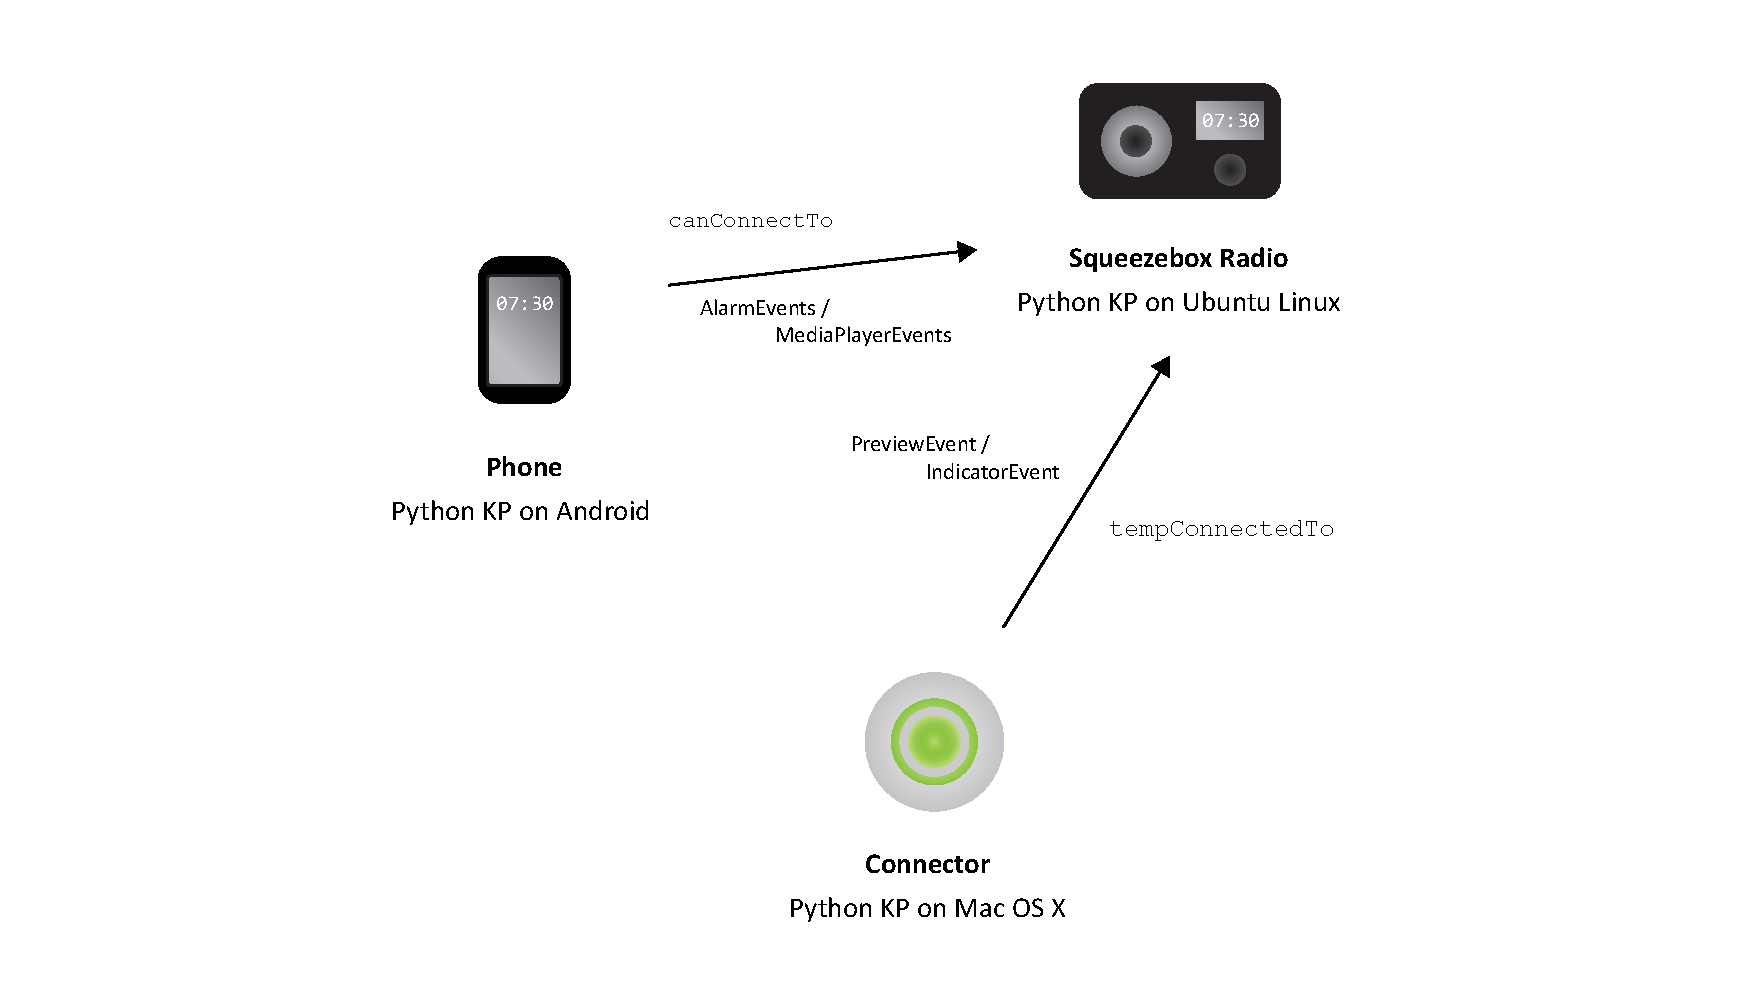
\includegraphics[width=450px]{functionalPreview1}}
\caption{Temporary connections for a \texttt{PreviewEvent} when source and sink are directly connected}
\label{functionalPreview1}
\end{figure}

\begin{figure}
\centerline{
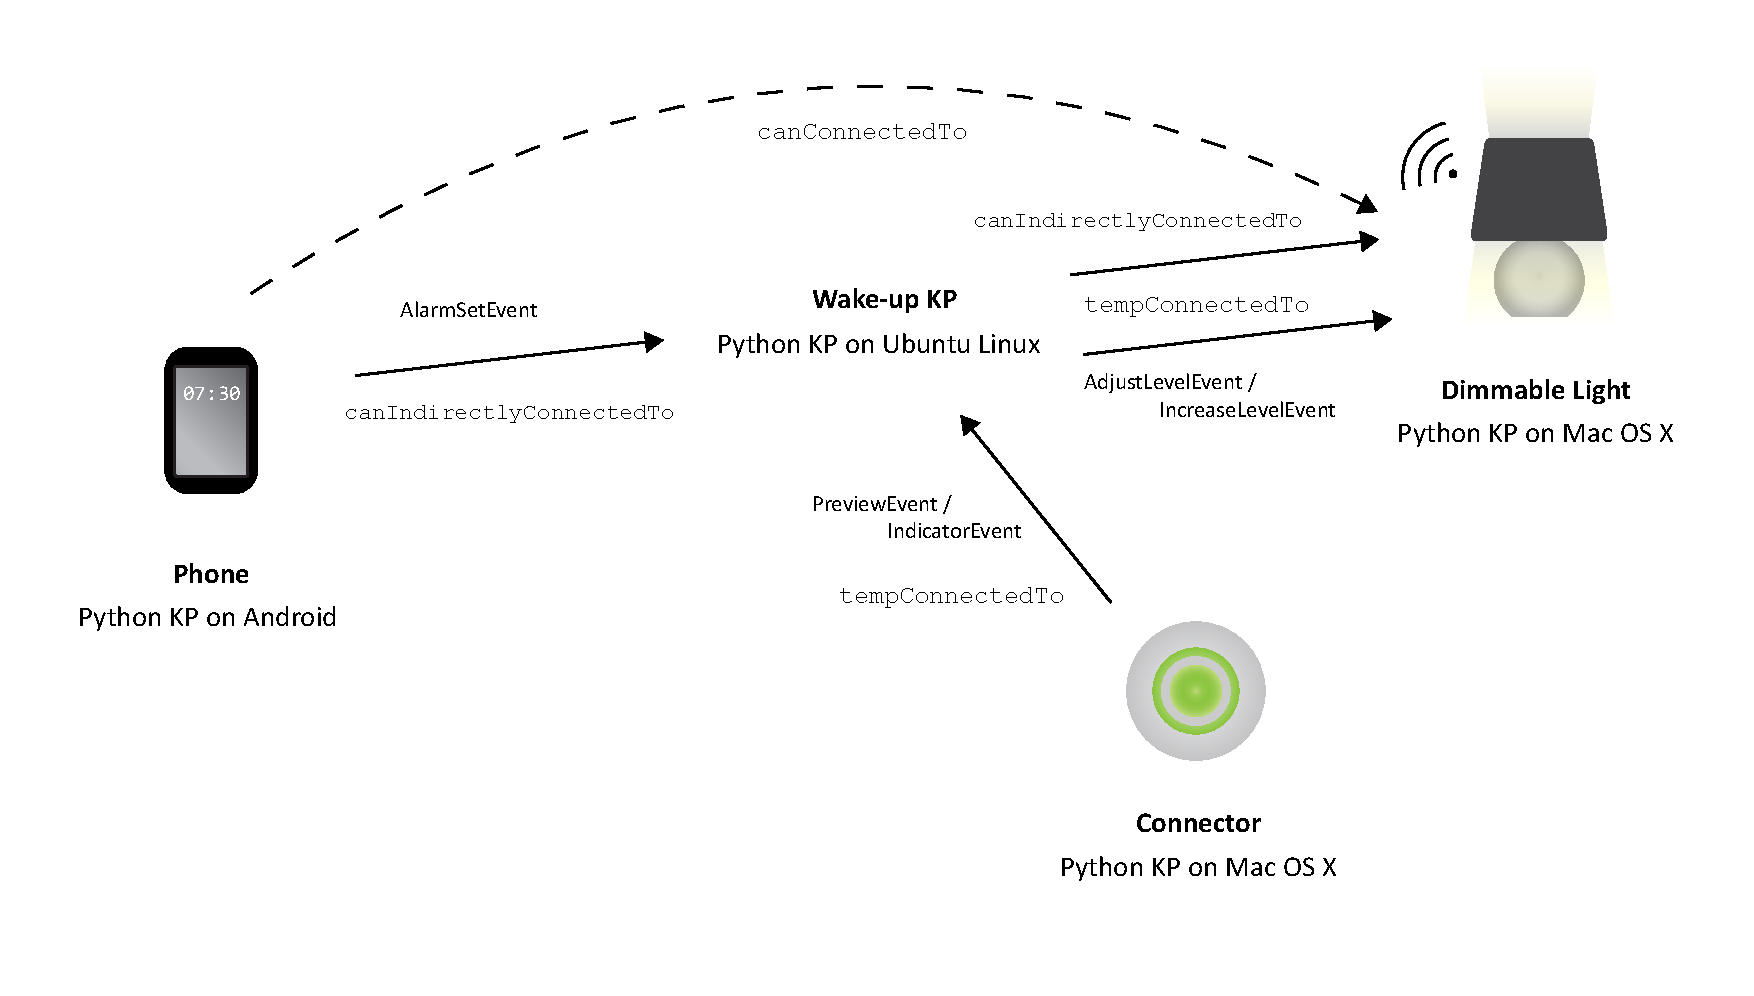
\includegraphics[width=450px]{functionalPreview}}
\caption{Temporary connections for a \texttt{PreviewEvent} when source and sink are connected via a semantic transformer}
\label{functionalPreview}
\end{figure}

\subsubsection{Functional feedback}
In many cases functional feedback of a semantic connection is trivial, for example hearing sound from a speaker that was just connected to a media player, or seeing photos on a TV when it is connected to a smart phone. However, functional feedback may only be available at another place or at another time. If we for instance take the example of synchronising a phone's alarm with the alarm radio, the real functional result may be hearing the radio play a song at the alarm time that was set on the phone. 

In such cases, the interaction designers should use augmented feedback as an \emph{indicator} that the alarm time was successfully set. When a semantic connection exists between a source and a sink, actions at the source should also be indicated at the sink. 

If the source and sink objects are in different locations, interaction designers should make sure that feedback is visible for a prolonged time period, or until it is dismissed by the user. This is to ensure that the indicator of the performed action will be noticed by the user. For the same reason, the order of connecting two spatially separated objects together is important, ensuring that establishing the connection happens in proximity of the sink, so that the feedback can be observed. 

\begin{example}
When music is playing on the phone and a connection is made between the phone and the internet radio, functional feedback is immediately given: the internet radio starts playing the same music, and an image of the album cover is displayed. The music on the source (phone) is muted, as the music playing on the internet radio is of a higher fidelity, and both share the same physical space. Context information, such as place/location, can be used to infer the correct behaviour.
\end{example}

\subsubsection{Augmented feedback} 
If there is no immediate link between action and function  (e.g. functional result is delayed, information is given about an internal state change), augmented feedback can be used to provide this information. We use an \texttt{IndicatorEvent} to provide augmented feedback when smart object is connected and there is no immediate functional feedback, e.g. a sink ``beeping'' when the alarm is set on the source.  The type of feedback required depends on the functionality of the connection. It is important for the feedback to coincide in time and modality with the event generated, as to maintain the causal link that is perceived by the user.

When a connections exists and an action performed on the source that has no immediate functional feedback, augmented feedback is provided to serve as an indicator. This feedback is  provided by the smart objects that are connected, in the modality that is supported by their interaction capabilities. Designers should aim for maintaining the modality of the augmented information across the smart objects. Additionally, ensuring that the feedback occurring at distributed objects coincide in time may strengthen the perceived causality of the link. Indicator events may also be used to indicate existing connections, e.g. when a user wishes to see what smart objects are currently connected to a source.  

\begin{example}
When the phone is connected to the internet radio and the internet radio is connected to the dimmable lamp, both the internet radio and the lamp gives augmented feedback when an alarm is set. The internet radio displays the alarm-set screen, confirming the alarm time and the dimmable lamp slowly flashes, to indicate that they are both connected and that the action on the source is confirmed.
\end{example}

%end TiiS



%\subsubsection{The Connector object}
%
%TODO Explain Connector functionality
%
%\begin{figure}[bth]
%\begin{msc}
%msc {
%	//hscale = "1.5";
%	
%    connector [label="Connector Object"], sib [label="SIB"];
%    connector=>connector [label="Scan first smart object"];
%    connector->sib [label="Retrieve name from tag"];
%    sib->connector [label="Name of first smart object"];
%    connector=>connector [label="Scan second smart object"];
%    connector->sib [label="Retrieve name from tag"];
%    sib->connector [label="Name of second smart object"];
%    connector->sib [label="Are they connected?"];
%    sib->connector [label="Not connected"];
%    connector->sib [label="Can they be connected?"];
%    sib->connector [label="Connection possible"];
%}
%\end{msc}
%        \caption{Connecting two devices using the Connector object}
%        \label{connectorSequence}
%\end{figure}



%\section{Evaluation}

% The sleep use case acted as an evaluation of the completeness and applicability of our semantic connections theory, evaluating whether: (a) the defined concepts in our theory are sufficiently defined to use them to implement the required functionalities, (b) the defined concepts can be used universally (for different use cases) and (c) the defined concepts form a complete set to describe the behaviour of semantic connections. Additionally, the implementation served as an example of how our theory can be used in a relevant and contemporary setting. We describe implementation details of how the concepts of the theory are modelled and conclude with changes and additions to the theory that were deemed necessary. 


\section{Discussion \& Conclusion}


% \subsection{Mismatches between device states}
% 
% Interaction events (Chapter \ref{EventModelling}) cause device state changes. When smart objects are interconnected, mismatches in device states may occur, as not all interaction events cause the same state transitions in all smart objects. The design decision to describe the interactions in terms of events as opposed to states was based on the idea that states can be logically inferred from events. Exchanging the events still leaves some autonomy to the smart object (or its developer) to decide what to do with the event. However, only sharing events is not always enough to create consistent behaviour. 
% 
% It is the responsibility of the source to communicate all state changes in the form of events, in order for the sink to keep in sync. Even then, it is still possible for two smart objects to be in different states while connected. Consider the case where the mobile phone is connected to the internet radio, sharing both alarm and music functionality. The user opens the music player on the mobile phone and presses Play, which causes the music to play back on the internet radio. As shown in Figure \ref{fsmPlayAlarm}, an \texttt{AlarmAlertEvent} generated by the mobile phone will cause the internet radio to go into an \texttt{Alarm} state. When the alarm is dismissed on the mobile phone, the internet radio will go into a \texttt{Pause} state, as this is the default behaviour when the alarm is dismissed on the internet radio itself. The mobile phone, however, is now in the \texttt{Play} state. To prevent this state mismatch, the mobile phone should not only send the \texttt{AlarmDismissEvent} that was generated through the user interaction, but also a \texttt{PlayEvent} to indicate that it is now playing music again.
% 
% 
% \begin{figure}[bth]
% %\begin{dot2tex}[dot,options=-tmath --autosize --cache]
% %digraph G {
% 	\digraph[scale=0.5]{MyGraph}{
% 	%rankdir=LR;
% 	font="Ubuntu";
% 	compound=true;	
% 	subgraph cluster0 {
% 	label="Mobile Phone";
% 	alarm1 [label=Alarm];
% 	play1 [label=Play];
% 	pause1 [label=Pause];
% 	pause1 -> play1 [label=Play];
% 	play1 -> alarm1 [label=Alarm];
% 	alarm1 -> play1 [label=Dismiss];
% 	play1 -> pause1 [label=Pause];
% 	}
% 	subgraph cluster1 {
% 	label="Internet Radio";
% 	alarm2 [label=Alarm];
% 	play2 [label=Play];
% 	pause2 [label=Pause];
% 	pause2 -> play2 [label=Play];
% 	play2 -> alarm2 [label=Alarm];
% 	alarm2 -> pause2 [label=Dismiss];
% 	play2 -> pause2 [label=Pause];
% 	}
% 	play1 -> pause2 [ltail=cluster0, label=AlarmDismissEvent];
% 	}
% %\end{dot2tex}
%     \caption{State mismatch between phone and internet radio}
%    \label{fsmPlayAlarm}
% \end{figure}



%We encountered a problem with state mismatches in our sleep use case that resulted in unexpected behaviour. In this specific case, the mobile phone was connected to the internet radio, sharing both alarm and music functionality. If the user opens the music player on the mobile phone and presses Play, it causes the music to play back on the internet radio. Besides playing music, an alarm was also set. When the \texttt{AlarmAlertEvent} generated by the mobile phone occurs, both the phone and the internet radio go to an alarm state. Dismissing the alarm on the phone causes the internet radio to go into a \texttt{Pause} state, as this is the default behaviour when the alarm is dismissed on the internet radio itself. The mobile phone, however, is now in the \texttt{Play} state (although no audio is audible since the speakers of the phone are muted because of the connection to the internet radio). In order to play music again, the phone needs to be paused first, followed by pressing play, to get the device states back into sync. Figure \ref{FSMalarmDismiss} displays this behaviour using a finite state machine.


%To prevent this state mismatch, the mobile phone should not only send the \linebreak \texttt{AlarmDismissEvent} that was generated through the user interaction, but also a \texttt{PlayEvent} to indicate that it is now playing music again.


% \begin{figure}
% \centering
% 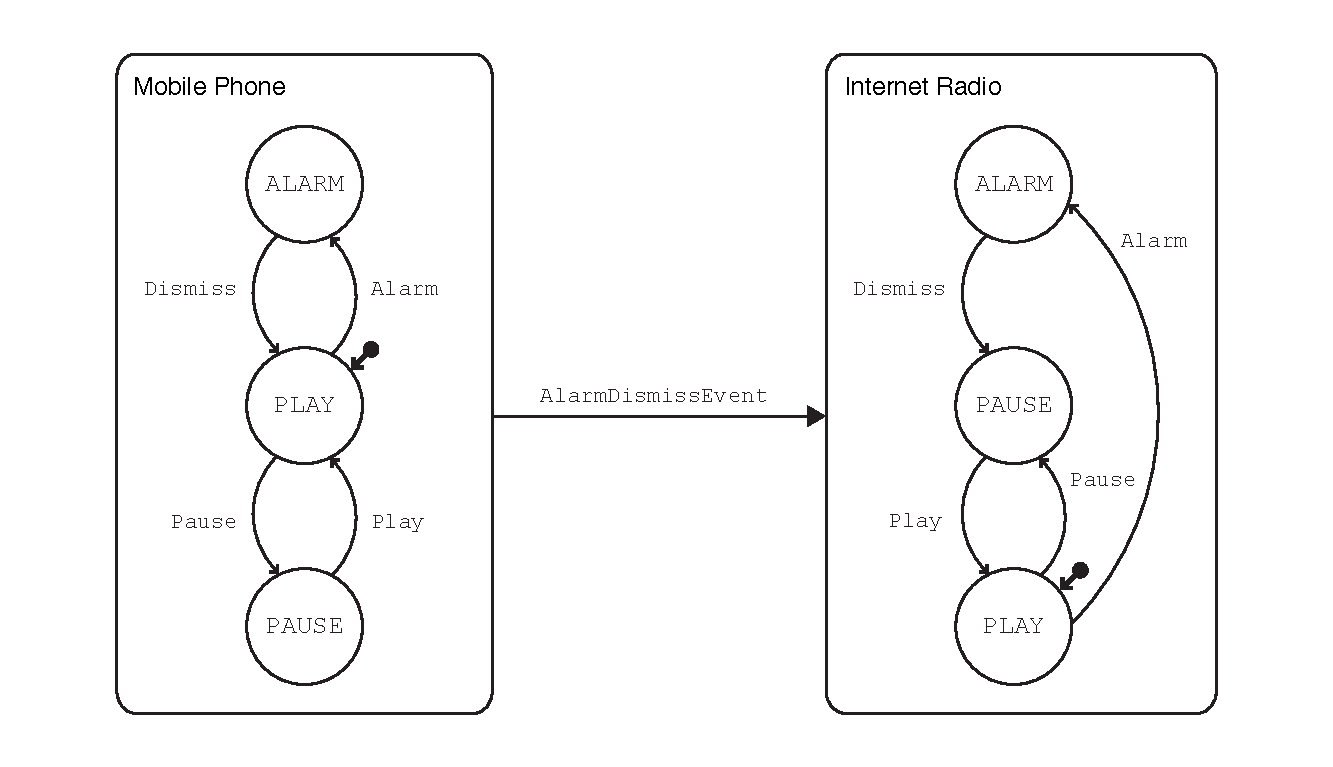
\includegraphics[width=400px]{FSMalarmDismiss}
% \caption{Finite state machine showing the state mismatch between phone and internet radio}
% \label{FSMalarmDismiss}
% \end{figure}


% (removed - Panos)
% \subsection{Setting time on devices}
% 
% For devices to interoperate with one another in a meaningful way, it is imperative that they have the same concept of time and that their clocks are synchronised. For something that should be very trivial, setting the time on devices is surprisingly difficult. Consider the devices we used in our last scenario:
% 
% \begin{itemize}
% 	\item The Zeo sleep manager does not allow for the time to be set remotely - it can only be set manually on the device itself.
% 	\item The Squeezebox radio retrieves the time from the server that it is connected to - you therefore need to be able to set the time on the computer running the server.
% 	\item On Android devices there are documented methods to set the time, e.g. \texttt{setCurrentMillis()}, but due to security restrictions non-system applications are not allowed to access these methods.
% \end{itemize}
% 
% Our workaround was to set the time on the Android phone, which will send the time value with a \texttt{TimeSetEvent}\marginpar{\texttt{TimeSetEvent} is a type of system event. For more information on system events, see Section \ref{SystemEvents}.} to the \texttt{SIB}. When a new \texttt{TimeSetEvent} is received, the Squeezebox KP updates the system time of the Squeezebox Server, requiring super user permissions. The Squeezebox is then restarted to synchronise the local time with that of the server.


%==Causes for increased reasoning time
%One example of where the reasoning time required increased to a number of seconds, was when we made use of the \texttt{owl:sameAs} property.


%\subsection{Conclusion}

The sleep use case acted as an evaluation of the completeness and applicability of the concepts and techniques described thus far. These approaches were distilled into a theory of semantic connections, which forms the basis of the next chapter. The implemented use case evaluated: 
\begin{itemize}
	\item whether the defined concepts and techniques are sufficiently defined to use them to implement the required functionalities;
	\item whether the defined concepts and techniques can be used universally (for different use cases); and
	\item  whether the defined concepts and techniques form a complete set to describe the behaviour of semantic connections.
\end{itemize}

Additionally, the implemented use case can serve as an example of how the theory described in the next chapter is used in a relevant and contemporary setting.

We consider the length of the verbal descriptions in Section \ref{D3Implementation} above to become unwieldy when describing more complex situations. There is a clear need for some kind of diagram notation to describe these situations. In the next chapter we introduce a theory of semantic connections that was created to help solve this problem. We first describe the concepts that are central to this theory, and then introduce a diagram notation based on \acp{FSM}, that can be used to model and explain the different concepts and situations.


